% METODOLOGIA------------------------------------------------------------------

\chapter{Construção do Protótipo}
\label{chap:prototipo}

Este capitulo descreve a montagem do protótipo para testes. Será feita uma introdução do funcionamento geral, e suas principais características. Posteriormente será mostrado o funcionamento da base de testes da câmera, conexões entre os servo motores e os pinos GPIO, instalação e configuração do sistema operacional para o Raspberry Pi, e desenvolvimento do programa e controle dos servo motores, desenvolvimento do aplicativo Android, responsável por capturar dados dos sensores de posição e envio pela rede sem fio.

\section{Especificação do Projeto}
\label{sec:especificacao}

Apesar de ser composta por diversos módulos, o projeto pode ser dividido conceitualmente em duas partes, denominados por módulo de coleta de dados, ou celular Android, e módulo de controle de câmera, ou Raspberry Pi. O módulo de controle de câmera é responsável por receber os dados de posição através de uma conexão socket, converter o sistema de coordenadas, aplicar um filtro para evitar o acionamento desnecessário dos motores e acionar os servos. O módulo de coleta de dados é responsável por configurar os sensores de localização disponíveis no smartfone, aplicar os filtros necessários para minimizar ruídos na coleta de dados e enviá-los através de uma conexão socket para o módulo de controle de câmeras. O funcionamento integrado dos módulos é ilustrado na \autoref{fig:diagrama_blocos} \par

\begin{figure}[H]
	\centering
	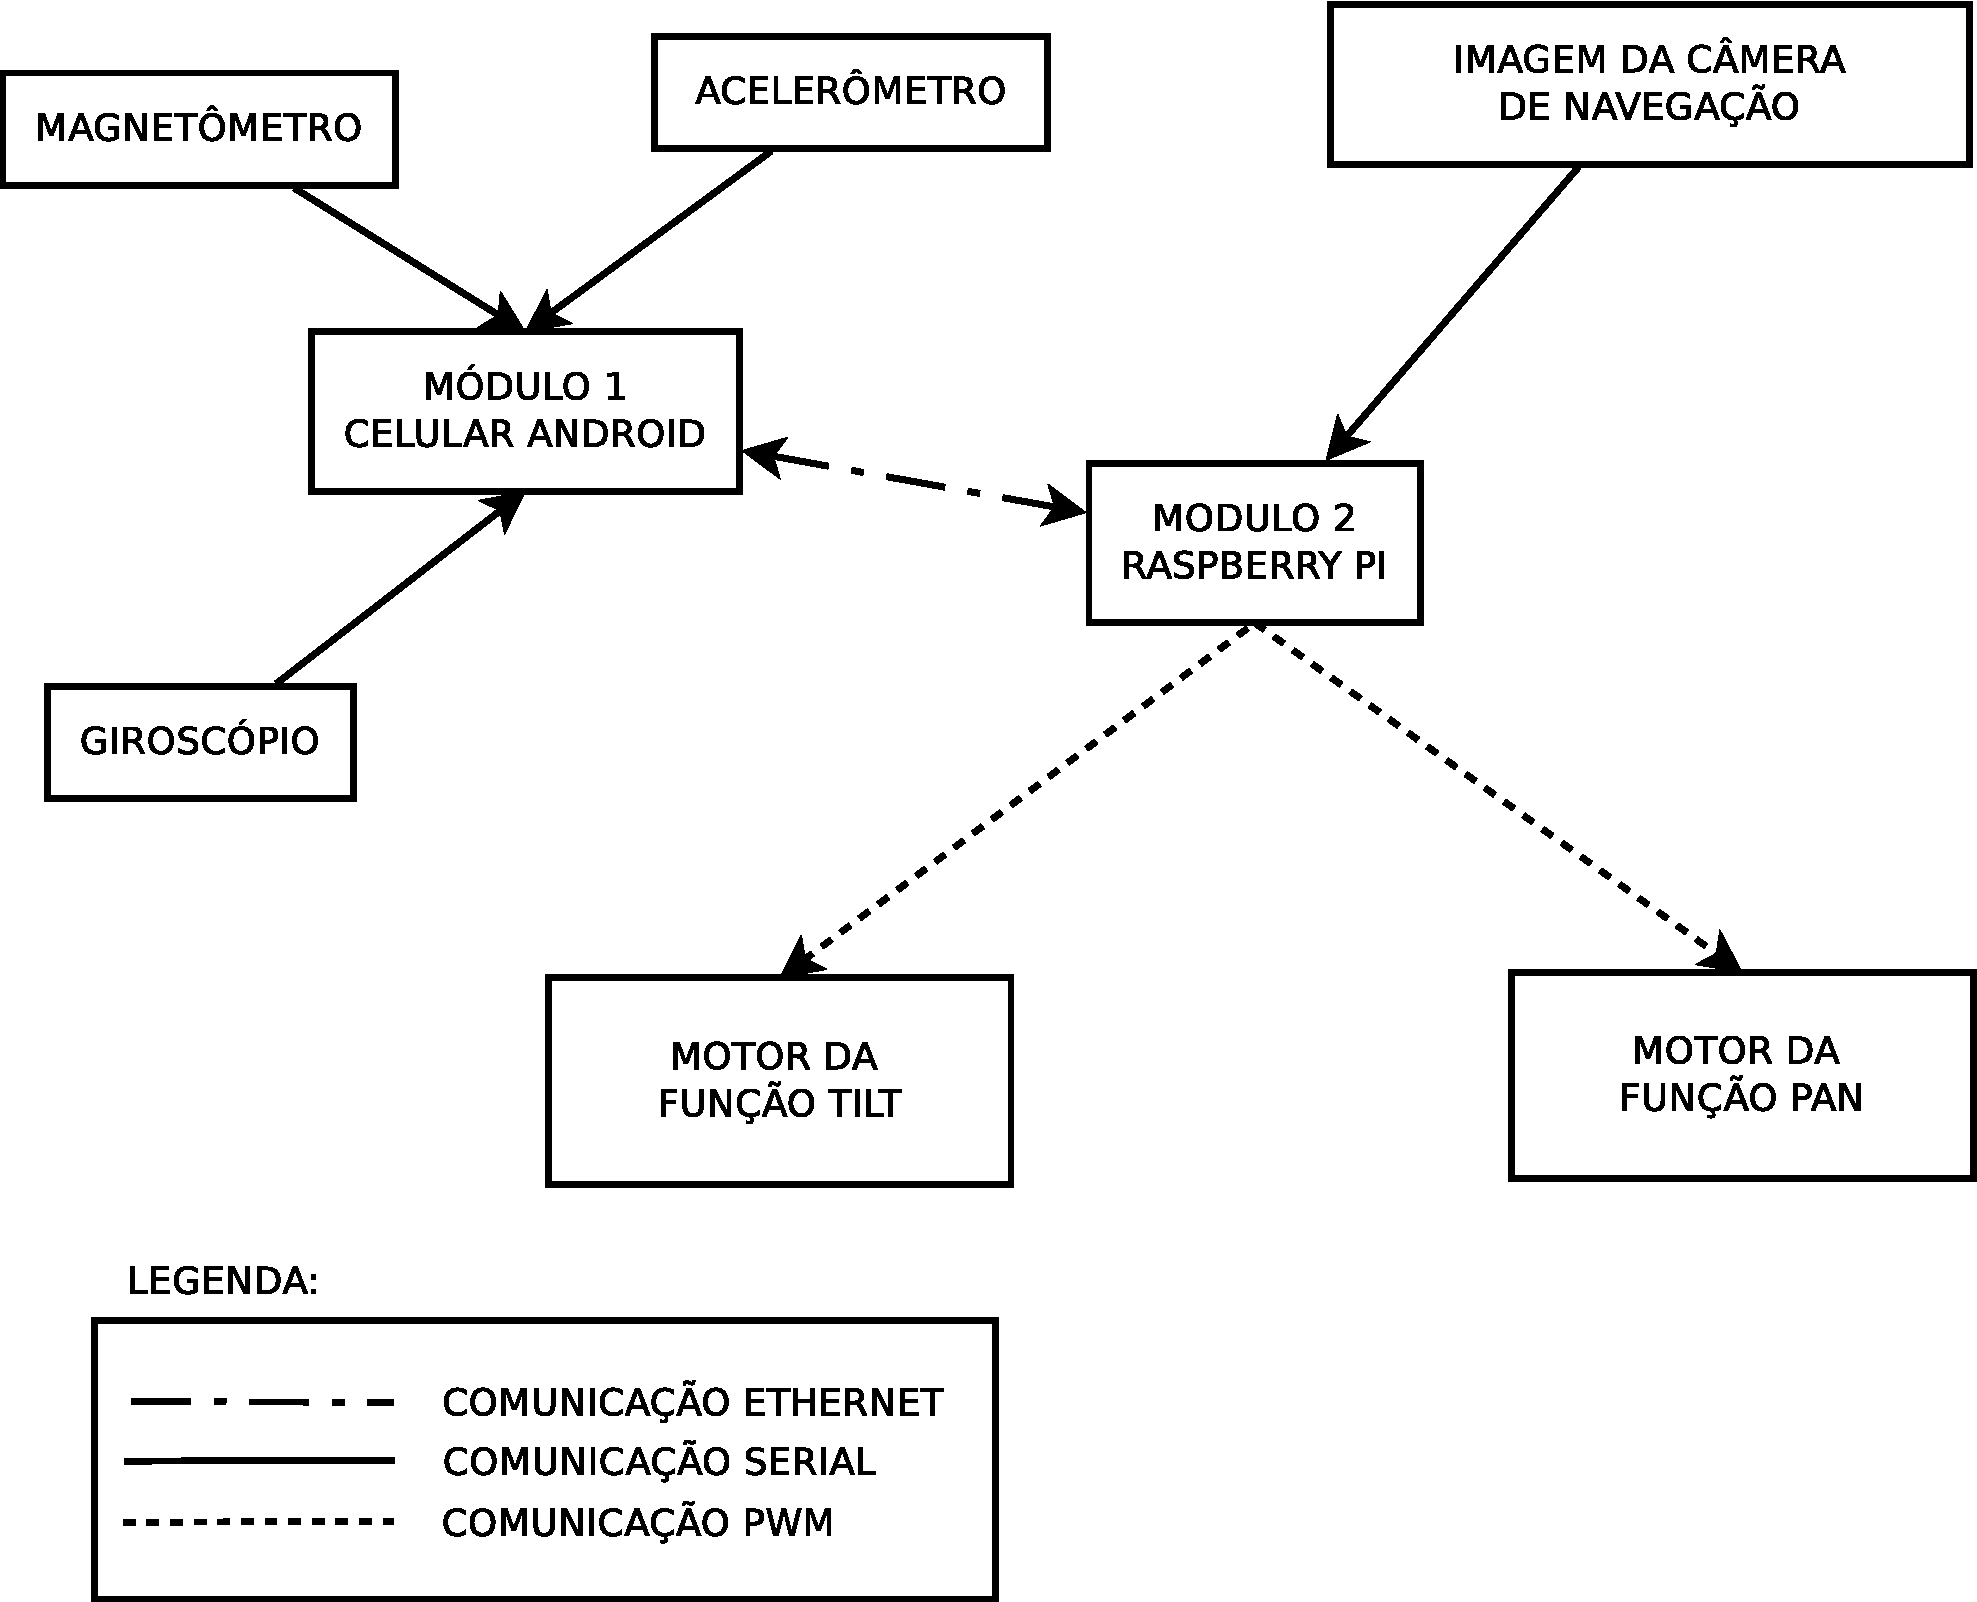
\includegraphics[width=0.9\textwidth]{figuras/diagrama-modulos-eps-converted-to.pdf}
	\caption{Diagrama de blocos da comunicação entre os módulos}
	\label{fig:diagrama_blocos}
\end{figure}